\documentclass{article}

\usepackage{fancyhdr}
\usepackage{ragged2e}
\usepackage{graphicx}
\usepackage{caption}
\usepackage{geometry}
\usepackage{amsmath}
\usepackage{rotating}

\usepackage{listings}
\usepackage{color}

\definecolor{dkgreen}{rgb}{0,0.6,0}
\definecolor{gray}{rgb}{0.5,0.5,0.5}
\definecolor{mauve}{rgb}{0.58,0,0.82}

\lstset{frame=tb,
  language=Java,
  aboveskip=3mm,
  belowskip=3mm,
  showstringspaces=false,
  columns=flexible,
  basicstyle={\small\ttfamily},
  numbers=none,
  numberstyle=\tiny\color{gray},
  keywordstyle=\color{blue},
  commentstyle=\color{dkgreen},
  stringstyle=\color{mauve},
  breaklines=true,
  breakatwhitespace=true,
  tabsize=4
}

\setcounter{secnumdepth}{1}

\usepackage{chngcntr}
\counterwithin{figure}{section}

\renewcommand*{\thepage}{C\arabic{page}}

\pagestyle{fancy}
\lhead{ACME Robotics}
\chead{\#8367}
\rhead{\ifcontents Contents \else Week \thesection \fi}

\newif\ifcontents
\contentstrue

\makeatletter
\renewcommand{\@seccntformat}[1]{}
\makeatother

\begin{document}\contentsfalse


\subsection{Sorting Mechanism}
%! Design a sorting mechanism to sort the minerals. 
Ashlin, Aidan and Kelly worked on the process for sorting the cubes from the balls. The first idea was a mechanical sorting system that would function like a coin sorter, allowing the cubes to fall through while the balls rolled past. This design was discarded because it took too much space and was not consistent. A new sorting system involved a color sensor and a U shaped cup. In figure \ref{fig:Sorter Version 2} the new system is shown connected to a prototype robot. The cube or ball would roll into the U-cup and then be read by the color sensor. The U-cup would then rotate about 135 degrees clockwise or counterclockwise to deposit the cube or ball in the corresponding cartridge. This idea did not work because there were not available servos that could rotate the required 270 and the system required too much space. This failed sorting system led to a third sorting system that was based around version two but took up less space and did not have to rotate as much. The final design, figure \ref{fig:Final Sorting Mechnism}, allowed the ball or cube to go into the rotating circle part where it would be read by the color sensor and then a servo would rotate the circle part about 45 degrees clockwise or counterclockwise to deposit it in the corresponding cartridge. This system worked significantly better because it allowed there to be only 90 degrees of rotation needed by the servo, the process would be significantly shorter, and the whole system could be condensed to take up no more than a 6 inches.

\begin{figure}
    \centering
    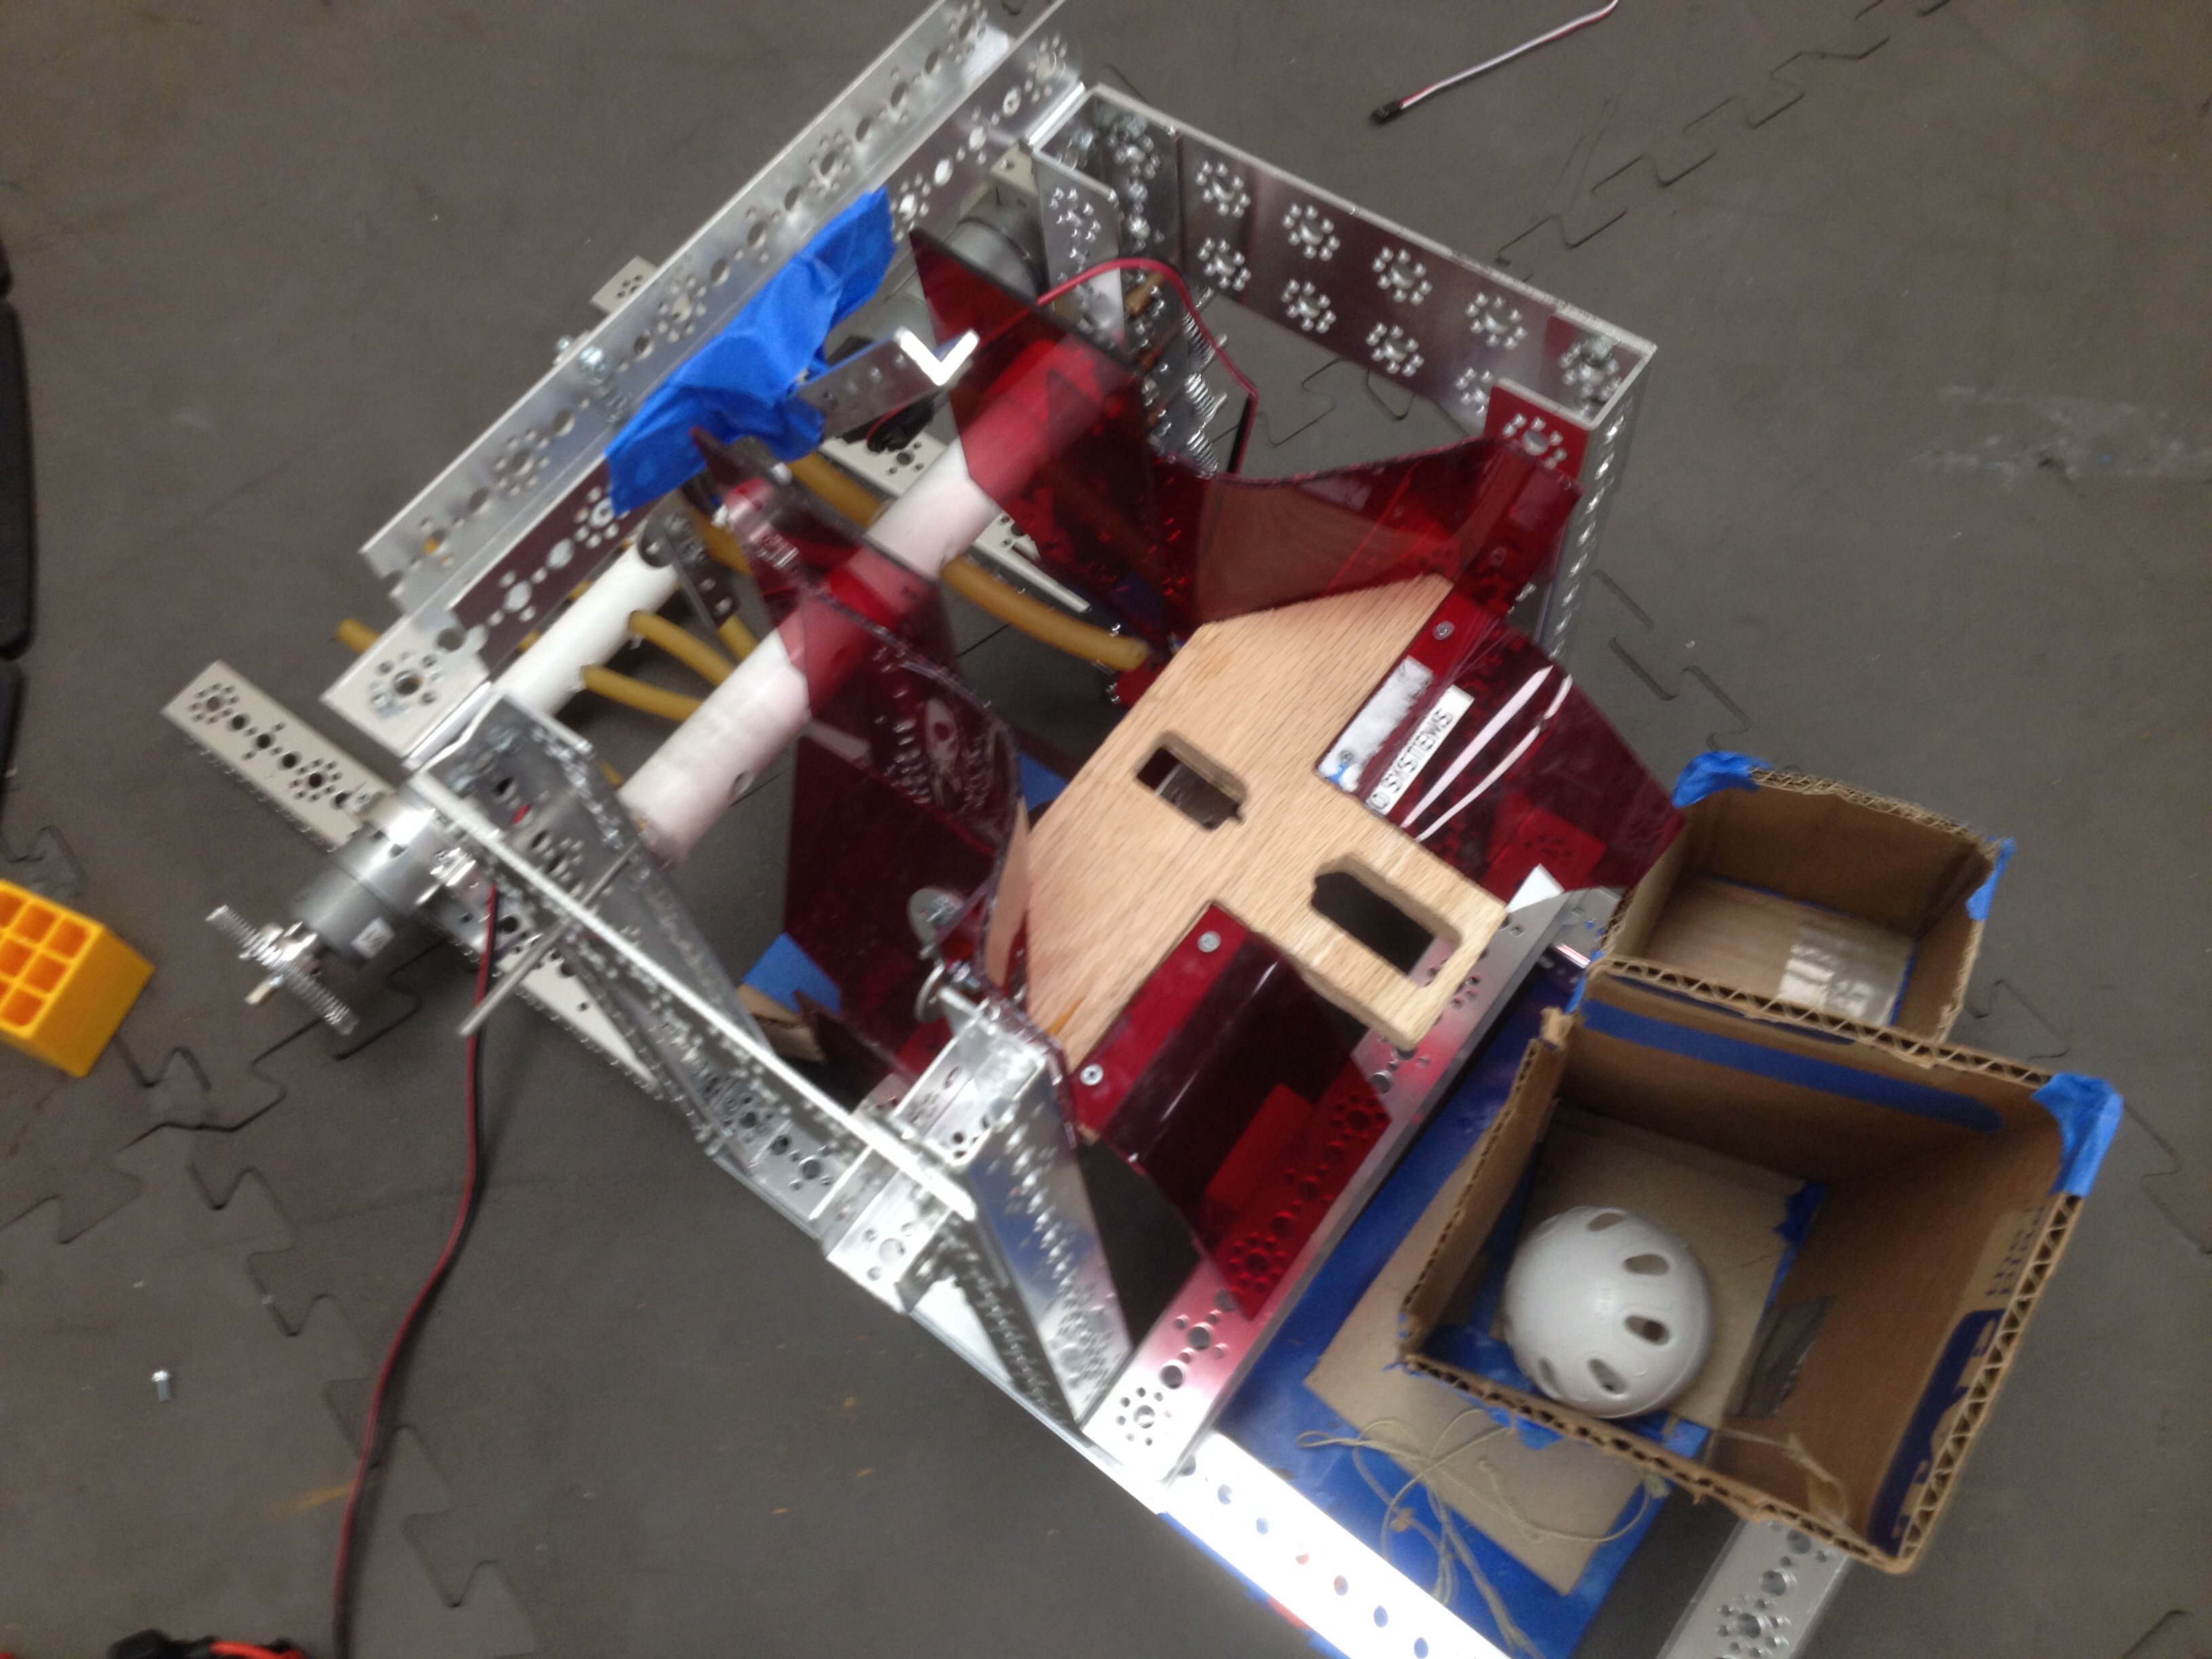
\includegraphics[width=.6\textwidth]{04_09-24/images/sorter.jpg}
    \caption{Sorter Version 2}
    \label{fig:Sorter Version 2}
\end{figure}

\begin{figure}
    \centering
    \includegraphics[width=.6\textwidth]{04_09-24/images/sorter2.png}
    \caption{Final Sorting Mechanism}
    \label{fig:Final Sorting Mechnism}
\end{figure}

\subsection{Investigate potential lift designs}
%! Figure out which lift designs would work the best for the robot. 
The lift is going to be one of the most important mechanisms on the robot this year, as it is required for both scoring and latching. It will also need to be capable of moving very quickly, when carrying minerals to the top of the lander, and powerful enough to lift the entire robot off the ground at the end of the match. Because the team had only used Rev linear motion kits and drawer slides before, Kelly investigated the other options available for linear motion. Any potential solution needed to be capable of extending to the top of the lander, which is 32 inches off of the surface of the field, which would require two 16 inch stages, or three shorter stages. Because the lander bracket is only about four inches above the top of the robot, the mechanism that will attach to the lander only needs to be mounted to the first stage, meaning that any subsequent stages do not need to be as robust, as they will only ever bear the weight of the scoring system, not the robot itself. These requirements are quite similar to the FRC challenge last year, Power Up, which required teams to lift blocks above their robot to score, and then hang from a bar. Team 254, in particular, had a design that is super promising. It consisted of two fixed rails, a box-like first stage than ran between the fixed rails, and a smaller second stage carriage that ran within the first stage frame. Since this overall form factor fit all of the requirements, the team decided to settle on it for now, and investigate hardware that it could be constructed from. Team 254 constructed their lift out of square aluminum tubing and bearings that would roll against the surface, making it super fast and smooth. While this provides the best performance, the main drawback to this approach is the difficulty in manufacturing the brackets that mount the bearings to the tubing to the tolerances necessary to make everything run smoothly. If any parts are out of alignment or not parallel, then it gets a lot harder to move the lift. Another pre-fabricated option that many teams used last year to extend their relic arms over the field wall is Actobototics x-rail. The x-rail has a v-shaped groove on each side of its cross-section, allowing a v-bearing to run in the track. This would cut down on the number of bearings needed for the lift, because each pair of bearings can constrain the lift in two dimensions, not just one. If the bearings are aligned so that the majority of the forces go radially into the bearings, rather than axially, than it could be quite robust. Kelly configured the lift using these parts, and then put together a list of parts necessary to construct the lift. Because the brackets are pre-fabricated, the tolerances are much tighter than could be achieved if the team manufactured them. 
\begin{figure}
    \centering
    \includegraphics[width=.75\textwidth]{04_09-24/images/lift.jpg}
    \caption{Lift concept sketches}
    \label{fig:lift}
\end{figure}

\subsection{Design lift gearbox}
%! Design a lift gearbox that can move the lift quickly and can lift up the robot. 
Another goal for the lift was finding a suitable gearbox that would fit all of the requirements for the lift. During this process, Kelly decided against a shifting gearbox because of the necessary complexity, which meant that at least two motors would need to be used to get sufficient torque to lift the robot at the gearing necessary to make the lift fast enough. A ratchet would also need to be involved so that the robot could hang from the lander without powering the motors, making it easier to start and end the match. After researching options for a dual-motor gearbox, Kelly settled on a Versa Planetary from VexPro, because it could use a dual motor input to drive one gearbox from two motors, removing the need to join the two motors after the reduction and was modular meaning any custom gear ratio could be created; it could also be integrated with a ratchet kit to allow for one-way rotation when lifting off the ground. After assuming that the robot would weigh the full 20 kg, and requiring the motor to be able to accelerate it at 2g, a 25:1 reduction would be necessary. This should be enough to lift the scoring mechanism to the top of the robot in 1.5s, so the gearbox should be sufficient. Kelly added the necessary parts to the order sheet.

\begin{figure}
    \centering
    \includegraphics[width=\textwidth, angle=90]{04_09-24/images/math.jpg}
    \caption{Lift gearbox math}
    \label{fig:my_label}
\end{figure}

\end{document}
